\section{Ziel}
Das Ziel dieses Versuchs ist es die Brennweite einer Linse mit verschiedenen Methoden zu messen. Außerdem sollen die Linsengleichung und das Abbildungsgesetz verifiziert werden.

\section{Theorie}
\label{sec:Theorie}

Linsen bestehen im Allgemeinen aus einem Material, das dichter als Luft ist.
Nach Fresnels Brechungsgesetzen wird das Licht beim Ein- und Austritt gebrochen.

\noindent In diesem Versuch werden Sammellinsen und Zerstreuungslinsen verwendet. Sammellinsen sind in der Mitte dicker als am Rand und bündeln das einstrahlende Licht. Die Brennweite $f$ einer Sammellinse, also die Entfernung von der Linse und dem Brennpunkt $F$, und die Bildweite $b$ sind, wie in Abb. \ref{sammellinse} zu erkennen, positiv und es entsteht ein reelles Bild auf einem Schirm.

\noindent Bei Zerstreuungslinsen (Abb. \ref{streulinse}) sind die Brennweite $f$ und die Bildweite $b$ negativ und ein virtuelles Bild wird erzeugt.

%Skizze dünne Sammellinse
\begin{figure}
    \centering
    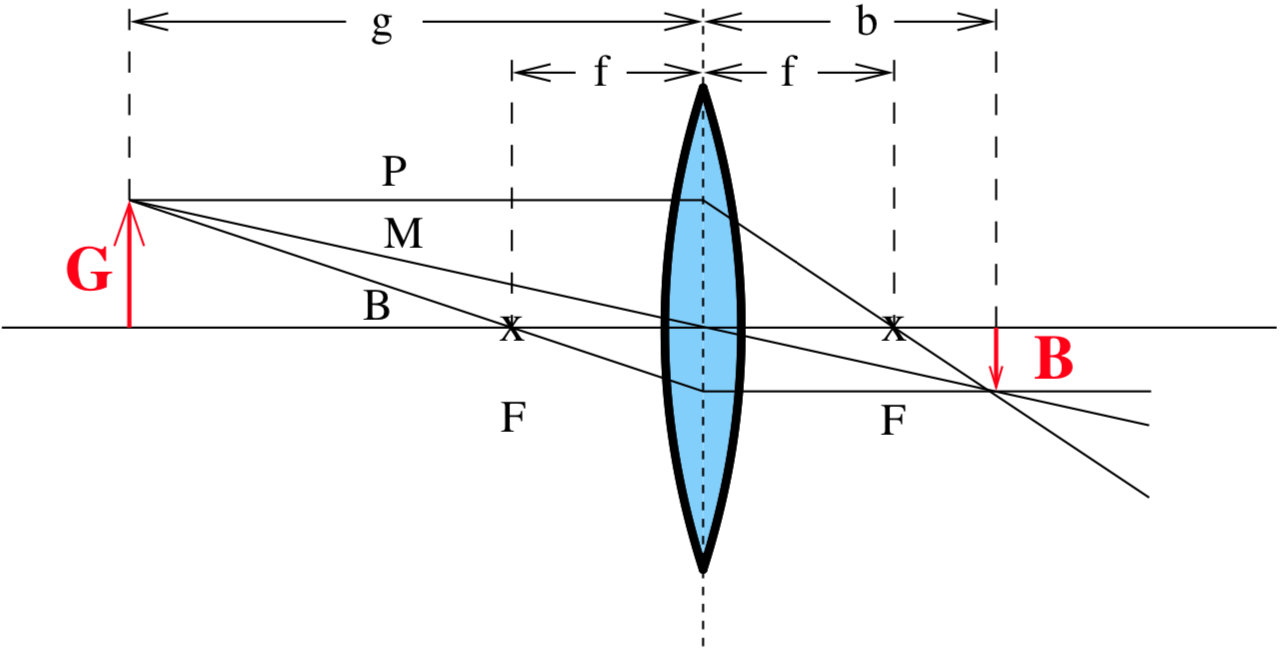
\includegraphics[width=8cm, height=5cm]{build/sammellinse.png}
    \caption{Skizze einer Sammellinse. Es sind die Gegenstandsgröße $G$, Gegenstandsweite $g$, Bildgröße $B$, Bildweite $b$, Brennpunkte $F$, Brennweiten $f$, Parallelstral $P$, Mittelpunktsstrahl $M$ und Brennpunktsstrahl $B$ eingezeichnet. \cite{V408}}
    \label{sammellinse}
\end{figure}

%Skizze dünne Streulinse
\begin{figure}
    \centering
    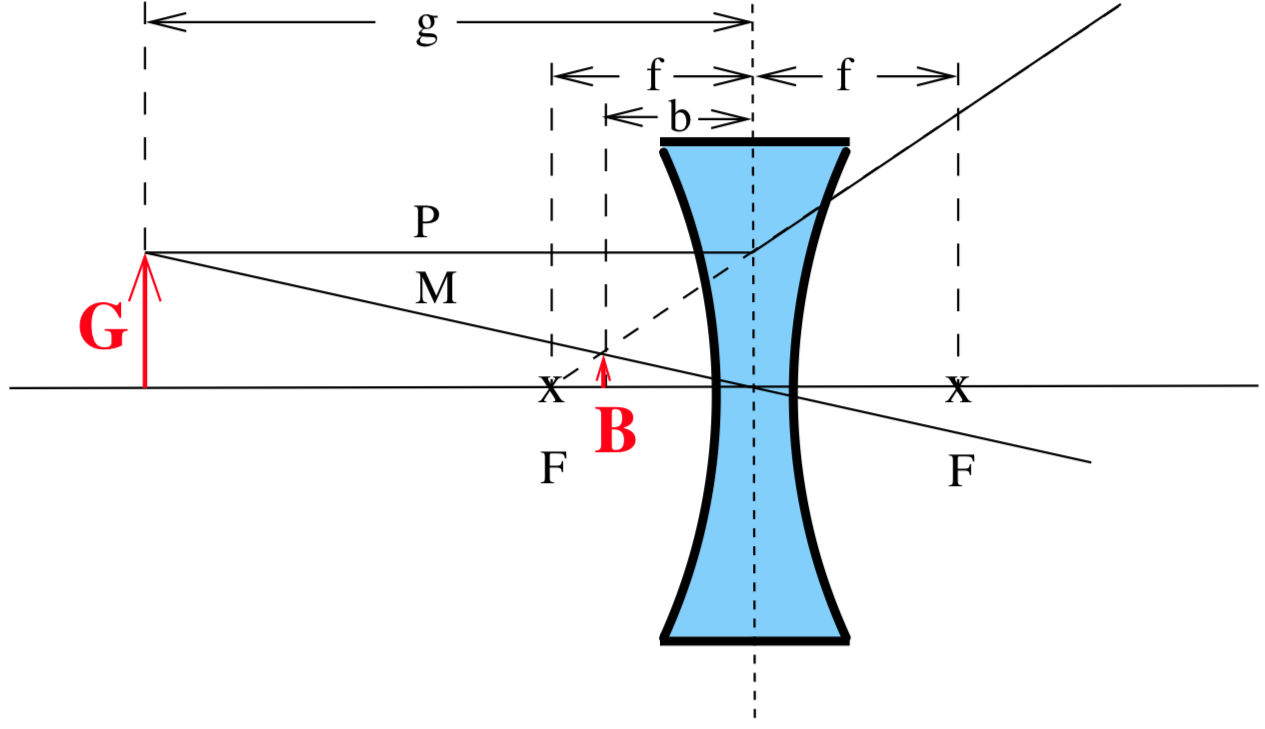
\includegraphics[width=8cm, height=5cm]{build/streulinse.png}
    \caption{Skizze einer Zerstreuungslinse. Es sind die Gegenstandsgröße $G$, Gegenstandsweite $g$, Bildgröße $B$, Bildweite $b$, Brennpunkte $F$, Brennweiten $f$, Parallelstral $P$ und Mittelpunktsstrahl $M$ eingezeichnet. \cite{V408}}
    \label{streulinse}
\end{figure}

\noindent Für die Bildkonstruktion in den Skizzen werden jeweils drei ausgezeichnete Strahlen eingezeichnet. Dabei gibt es den Parallelstrahl $P$, den Mittelpunktsstrahl $M$ und den Brennpunktsstrahl $B$. Die Wortbedeutung ist selbsterklärend.

\noindent Aus den Brechungsgesetzen und einigen geometrischen Überlegungen folgt das sogenannte Abbildungsgesetz
\begin{equation}
    V = \frac{B}{G} = \frac{b}{g}.
    \label{eqn:abbildungsgesetz}
\end{equation}
\noindent Dabei ist $V$ der Abbildungsmaßstab, also das Verhältnis zwischen Bild- und Gegenstandsgröße, $B$ die Bildgröße und $G$ die Gegenstandsgröße. Im selben Verhältnis stehen $b$, die Bildweite, und $g$, die Gegenstandsweite, zueinander. 

\noindent Für dünne Linsen folgt aus denselben Überlegungen die Linsengleichung 
\begin{equation}
    \frac{1}{f}= \frac{1}{b} + \frac{1}{g}.
    \label{eqn:linsengleichung}
\end{equation}

\noindent Bei Systemen aus mehreren Linsen muss die Rechnung anders gemacht werden. 
Die Mittelebene muss dann durch zwei Hauptebenen $H$ und $H'$ ersetzt werden.
Brennweite, Gegenstandsweite und die Bildweite werden in Bezug zu der jeweiligen Hauptebene bestimmt, die man stellvertretend für das ganze Linsensystem betrachtet. 

\noindent Die sogenannte reziproke Brennweite definiert die Brechkraft als $D= 1/f$ mit der Einheit Dioptrie. Bei einem Linsensystem aus verschiedenen gekrümmten Linsen summieren sich die Brechkräfte $D_i$, der einzelnen Linsen, sodass gilt 

\begin{equation*}
    D= \sum{i}^N D_i.
    \label{eqn:brechungskraft}
\end{equation*}


\subsection{Abbildungsfehler}
Es gibt Abbildungsfehler, die die Messung und vor allem die Exaktheit der Messung beeinflussen können. So liegt zum Beispiel bei der sogenannten spährischen Abberration der Brennpunkt achsenferner Strahlen näher an der Linse als der von achsennahen Strahlen. 

\noindent Bei der chromatischen Abberation liegt der Brennpunkt von blauem Licht näher an der Linse als der von rotem Licht, da blaues Licht aufgrund der Dispersionsrelation stärker gebrochen wird.  
%Anderen beiden Abbildungsfehler auch beschreiben


\subsection{Methode von Bessel}
Die Brennweite wird mit einer Linse bestimmt, indem der Abstand zwischen Gegenstand und Bild konstant bleibt und zwei Linsenpositionen gesucht werden, bei denen das Bild scharf ist. Aus der Summe 
\begin{equation}
    e = g_1 + b_1 = g_2 + b_2
    \label{eqn:e}
\end{equation}
und der Differenz 
\begin{equation}
    d = g1- b1 = g2 - b2
    \label{eqn:d}
\end{equation}
ergibt sich die Brennweite zu
\begin{equation}
    f = \frac{e^2 - d^2}{4 e}.
    \label{eqn:fbessel}
\end{equation} 

\begin{figure}
    \centering
    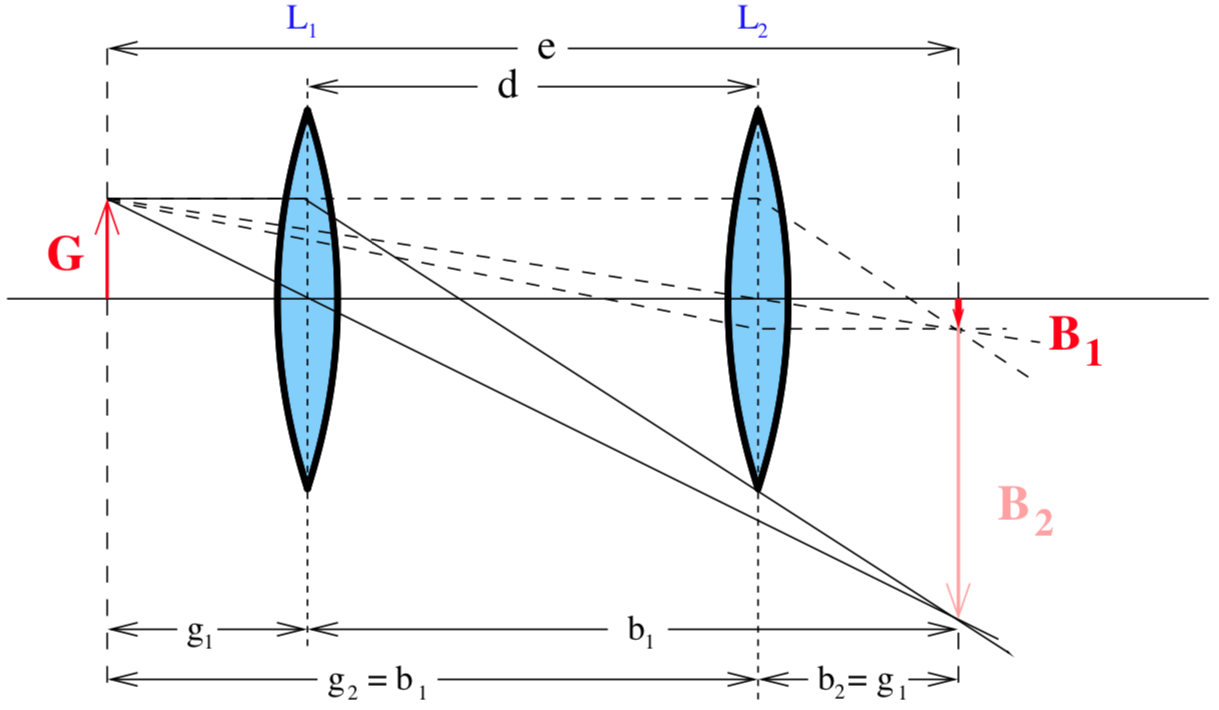
\includegraphics[width=8cm, height=5cm]{build/bessel.png}
    \caption{Skizze der Methode von Bessel. Es sind zwei Linsen zu sehen, die die zwei Linsenpositionen darstellen sollen. Es sind außerdem die Gegenstandsgröße $G$, Gegenstandsweiten $g_\text{i}$, Bildgröße $B$, Bildweiten $b_\text{i}$, Abstand zwischen Gegenstand und Bild $e$, Abstand der Linsenpositionen $d$, Parallelstral $P$, Mittelpunktsstrahl $M$ und Brennpunktsstrahl $B$ eingezeichnet. \cite{V408}}
    \label{fig:bessel}
\end{figure}

\subsection{Methode von Abbe}
Ein Linsensystem aus einer Sammel- und einer Zerstreuungslinse wird zwischen Schirm und Lampe hin- und herbewegt und es wird nach einem scharfen Bild gesucht. Der Aufbau ist in Abb. \ref{fig:abbe} zu sehen.
Die Gegenstandsweite $g'$ und die Bildweite $b'$ lassen sich bei einem System aus Linsen von einem Referenzpunkt aus gut messen. 
Wenn der Abbildungsmaßstab bekannt ist, lässt sich daraus die Brennweite und der Abstand zu den Hauptebenen bestimmen. 
Dafür kann der lineare Zusammenhang 
\begin{equation}
    g' = g + h = f \cdot \left(1 + \frac{1}{V} \right) + h
    \label{eqn:gstrich}
\end{equation}
beziehungsweise der Zusammenhang 
\begin{equation}
    b' = b + h' = f \cdot \left(1 + V \right) + h'
    \label{eqn:bstrich}
\end{equation}
mit einer linearen Regression gelöst werden. 
Dabei sind $h$ der Abstand von Referenzpunkt und Hauptebene $H$ und $h'$ der Abstand von Referenzpunkt und Hauptebene $H'$.

\begin{figure}
    \centering
    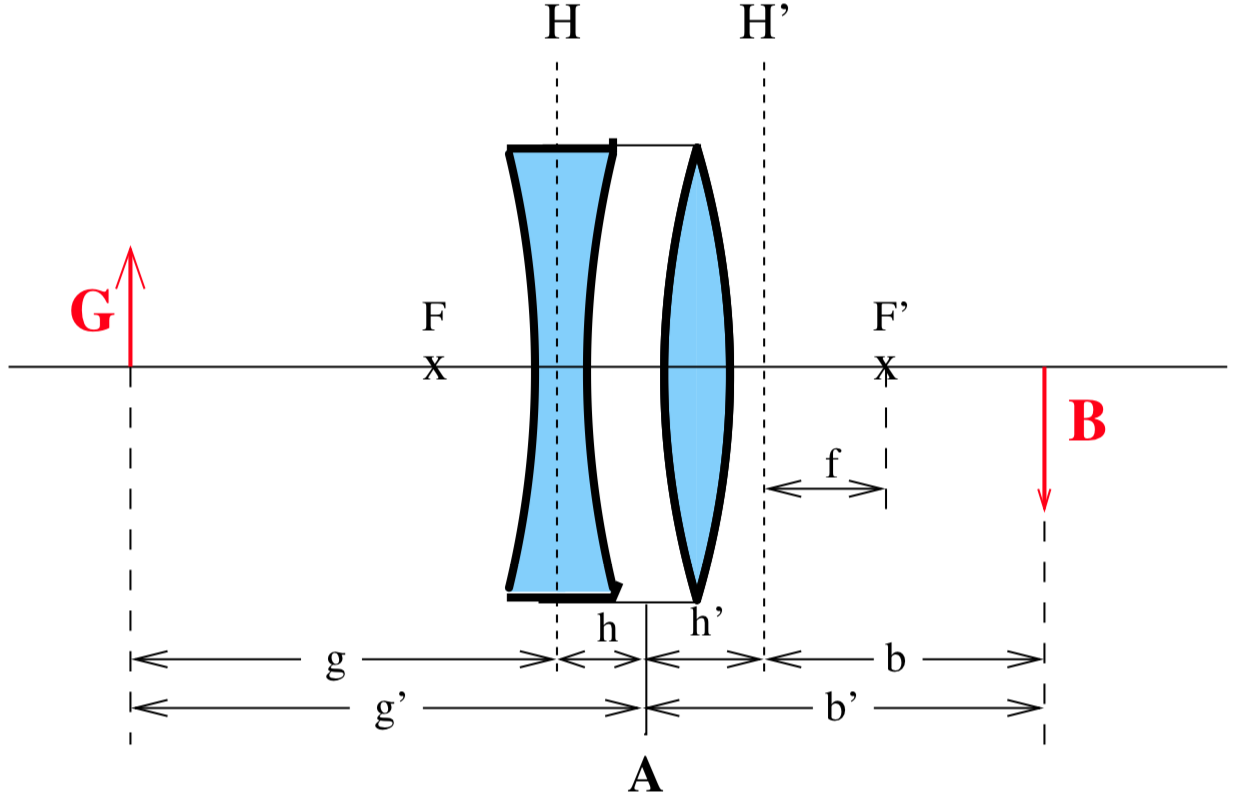
\includegraphics[width=8cm, height=5cm]{build/abbe.png}
    \caption{Skizze der Methode von Abbe. Es sind eine Sammel- und eine Zerstreuungslinse zu sehen. Außerdem sind die Gegenstandsgröße $G$, Gegenstandsweite $g$, Bildgröße $B$, Bildweite $b$, der Referenzpunkt $A$, die Gegenstandsweite $g'$ bezüglich des Referenzpunktes, die Bildweite $b'$ bezüglich des Referenzpunktes, Brennpunkte $F$, Brennweite $f$, die Hauptebenen $H$ und $H'$ sowie die Abstand $h$ und $h'$ von Referenzpunkt zu den Hauptebenen eingezeichnet. \cite{V408}}
    \label{fig:abbe}
\end{figure}
